%%%%%%%%%%%%%%%%%%%%%%%%%%%%%%%%%%%%%%%%%%%%%%%%%%%%%%%
% A template for Wiley article submissions.
% Developed by Overleaf. 
%
% Please note that whilst this template provides a 
% preview of the typeset manuscript for submission, it 
% will not necessarily be the final publication layout.
%
% Usage notes:
% The "blind" option will make anonymous all author, affiliation, correspondence and funding information.
% Use "num-refs" option for numerical citation and references style.
% Use "alpha-refs" option for author-year citation and references style.

\documentclass[alpha-refs]{wiley-article}
% \documentclass[blind,alpha-refs]{wiley-article}


%%%%%%%%%%%%%%%%%%%%%%%%%%%%%%%%%%%%%%%%%%%%%%%%%%%%%%%%%
%%%%%%%%%%% JDT:  Annotation Code %%%%%%%%%%%%%%%%%%%%%%%%%%%%%%%%%%
%%%%%%%%%%%%%%%%%%%%%%%%%%%%%%%%%%%%%%%%%%%%%%%%%%%%%%%%%

\usepackage{color}
\usepackage{ulem}

 % Uncomment to display with annotation; comment out otherwise
\newcommand{\add}[1]{\textcolor{blue}{#1}}
\newcommand{\delete}[1]{\textcolor{red}{\sout{#1}}}
\newcommand{\edit}[2]{\textcolor{red}{\sout{#1}} \textcolor{blue}{#2}}
\newcommand{\mnote}[1]{\marginpar{\textcolor{green}{\textbf{#1}}}}

 % Uncomment to display without annotation; comment out otherwise
%\newcommand{\add}[1]{#1}
%\newcommand{\delete}[1]{}
%\newcommand{\edit}[2]{#2}
%\newcommand{\mnote}[1]{}

%%%%%%%%%%%%%%%%%%%%%%%%%%%%%%%%%%%%%%%%%%%%%%%%%%%%%%%%%
%%%%%%%%%%%%%%%%%%%%%%%%%%%%%%%%%%%%%%%%%%%%%%%%%%%%%%%%%
%%%%%%%%%%%%%%%%%%%%%%%%%%%%%%%%%%%%%%%%%%%%%%%%%%%%%%%%%

% Add additional packages here if required
\usepackage{amsfonts,siunitx}

\usepackage[colorlinks,allcolors=blue]{hyperref}
\usepackage[ruled]{algorithm2e}
\SetArgSty{textnormal}

% Notation
\usepackage{enumitem, url}
\DeclareMathOperator{\E}{\mathbb{E}} % expectation
\newcommand{\Z}{\mathbb{Z}}
\newcommand{\R}{\mathbb{R}}
\newcommand{\N}{\mathbb{N}}
\newcommand{\C}{\mathbb{C}}
\newcommand{\blank}{\makebox[1ex]{\textbf{$\cdot$}}}
\newcommand\independent{\protect\mathpalette{\protect\independenT}{\perp}}
\def\independenT#1#2{\mathrel{\rlap{$#1#2$}\mkern2mu{#1#2}}}
\renewcommand{\phi}{\varphi}
\renewcommand{\epsilon}{\varepsilon}
\newcommand*\diff{\mathop{}\!\mathrm{d}}
\newcommand{\weakly}{\rightsquigarrow}
\newcommand\bigO{\ensuremath{\mathcal{O}}}
\newcommand{\midd}{\; \middle|\;}
\newcommand{\1}{\mathbb{1}}
\usepackage{ifthen} %% Empirical process with default argument
\newcommand{\G}[2][n]{
{\ensuremath{\mathbb{G}_{#1}}{\left[#2\right]}}
}
\DeclareMathOperator*{\argmin}{\arg\!\min}
\DeclareMathOperator*{\argmax}{\arg\!\max}
\newcommand{\data}{\ensuremath{\mathcal{D}}}
\newcommand{\sample}{\ensuremath{\mathcal{S}}}



% Update article type if known
\papertype{Original Article}
% Include section in journal if known, otherwise delete
\paperfield{Journal Section}

\title{The joint survival super learner: A super learner for right-censored
  data}


% Include full author names and degrees, when required by the journal.
% Use the \authfn to add symbols for additional footnotes and present addresses, if any. Usually start with 1 for notes about author contributions; then continuing with 2 etc if any author has a different present address.
\author[1]{Anders Munch}
\author[1]{Thomas A.~Gerds}

% \contrib[\authfn{1}]{Equally contributing authors.}

% Include full affiliation details for all authors
\affil[1]{Section of Biostatistics, University of Copenhagen}

\corraddress{Anders Munch, Section of Biostatistics, University of
  Copenhagen, 1355 Copenhagen, Denmark}
\corremail{a.munch@sund.ku.dk}

% \presentadd[\authfn{2}]{Department, Institution, City, State or Province, Postal Code, Country}

% \fundinginfo{Funder One, Funder One Department, Grant/Award Number: 123456, 123457 and 123458; Funder Two, Funder Two Department, Grant/Award Number: 123459}

% Include the name of the author that should appear in the running header
\runningauthor{Munch and Gerds}

\begin{document}

\maketitle

\begin{abstract}
  Risk prediction models are widely used to guide
  real-world decision-making in areas such as healthcare and
  economics, and they also play a key role in estimating nuisance
  parameters in semiparametric inference. The super learner is a
  machine learning framework that combines a library of prediction
  algorithms into a meta-learner using cross-validated loss. In the
  context of right-censored data, careful consideration must be given
  to both the choice of loss function and the estimation of expected
  loss.  Moreover, estimators such as inverse probability of censoring
  weighting require accurate modeling and an estimator of the
  censoring distribution. We propose a novel approach to super
  learning for survival analysis that jointly evaluates candidate
  learners for both the event-time distribution and the censoring
  distribution. Our method imposes no restrictions on the algorithms
  included in the library, accommodates competing risks, and does not
  rely on a single pre-specified estimator of the censoring
  distribution. We establish a finite-sample bound on the average
  price we pay for using cross-validation, and show that this price
  vanishes asymptotically, up to poly-logarithmic terms, provided that
  the size of the library does not grow faster than at a polynomial
  rate in the sample size. We demonstrate the practical utility of our
  method using prostate cancer data and compare it to existing super
  learner algorithms for survival analysis using synthesized data.

  % Please include a maximum of seven keywords
  \keywords{competing risks, cross-validation, loss based estimation,
    right-censored data, super learner}
\end{abstract}


\section{Introduction}
\label{sec:introduction}

Accurately predicting risk from time-to-event data is a central
challenge in various research fields, such as epidemiology, economics,
and weather forecasting, with applications in clinical decision making
and policy interventions. For instance, in prostate cancer management,
clinicians often need to estimate a patient’s risk of disease
progression and mortality over time to make informed decisions about
treatment strategies such as active surveillance versus immediate
intervention. Reliable risk prediction models can help tailor care to
individual patients, avoid overtreatment, and allocate healthcare
resources more effectively. Super learning \citep{van2007super}, also
known as ensemble learning or stacked regression
\citep{wolpert1992stacked,breiman1996stacked}, provides a powerful
approach to this problem by combining multiple candidate prediction
models to reduce the risk of bias incurred by a single potentially
mispecified model. In survival analysis, a super learner may for example combine a
stack of Cox regression models with a stack of random survival forests
\citep[][Section 8.4]{gerds2021medical}. Such a strategy has recently
produced \textit{KDpredict} (\url{https://kdpredict.com/}) a model which
jointly predicts the risks of kidney failure and all-cause mortality
at multiple time horizons based on different sets of covariates
\citep{liu2024predicting}. To evaluate the prediction performance of
the learners, the super learner behind KDpredict uses inverse
probability of censoring weighting (IPCW), where the censoring
distribution is estimated under the restrictive assumption that it
does not depend on the covariates. This is a potential source of bias
which is difficult to overcome with the currently available methods.

In this article, we propose the {\it joint survival super learner}, a
new super learner designed to handle the specific challenges of
ensemble learning with right-censored data. The joint survival super
learner simultaneously learns prediction models for the event-time and
censoring distributions. The joint survival super learner is based on
a competing risks model for the observed data, in which censoring is
included as a state of its own, such that at any time it is known in
which state an individual is. We assume conditionally independent
censoring and exploit well-known relationships between the observed
data distribution on the one side and the partly unobserved
distributions of the event time and the censoring time on the
other. Learners for the event-time and censoring hazard functions are
then assessed using the integrated Brier score across all states of
the observed data. Our estimation framework thus naturally
incorporates competing risks, avoids restrictive assumptions on the
censoring distribution, and produces an estimator for the censoring
distribution. Our approach is also fully flexible with respect to the
choice of learners. The latter is in contrast to other proposals which
restrict the library of learners to specific model classes
\citep{polley2011-sl-cens,golmakani2020super}, as we discuss in more
detail in Section~\ref{sec:super-learning}.

To analyse the theoretical properties of the joint survival super
learner, we focus on the discrete super learner, which selects the
model in the library with the best estimated performance
\citep{van2007super}. We provide theoretical guarantees for the
performance of the joint survival super learner, and in particular
show that the discrete joint survival super learner is consistent
when the library of learners includes at least one consistent
learner. We also derive a finite-sample oracle inequality for the
discrete joint survival super learner. We demonstrate how to construct
a library of learners using common methods for survival analysis and
illustrate the use of the joint survival super learner using a
prostate cancer data set.

The article is organized as follows. We introduce our notation and
framework in Section~\ref{sec:framework}.
Section~\ref{sec:super-learning} introduces loss-based super learning
and discusses other existing super learners for right-censored
data. In Section~\ref{sec:joint-survival-super-learner} we define the joint
survival super learner, while Section~\ref{sec:theor-results-prop}
provides theoretical guarantees. Section~\ref{sec:numer-exper} reports
the results of a series of numerical experiments, and
Section~\ref{sec:real-data-appl} illustrates the method on prostate
cancer data. We conclude with a discussion in
Section~\ref{sec:discussion}. Proofs are collected in the
Appendix. Code and an implementation of the joint survival super
learner in R \citep{R} are available at
\url{https://github.com/amnudn/joint-survival-super-learner}.

\section{Notation and framework}
\label{sec:framework}

In a competing risks framework \citep{andersen2012statistical} with
\(J\) competing risks, let \( T\) be a time to event variable,
\(D\in\{1,2,\dots,J\}\) the cause of the event, and $X \in
\mathcal{X}$ a vector of baseline covariates taking values in a
bounded subset \( \mathcal{X} \subset \R^p \), \( p\in\N \). Let
$\tau< \infty$ be a fixed prediction horizon. We use \(\mathcal{Q} \)
to denote the collection of all probability measures on \( [0,\tau]
\times \{1,2,\dots,J\}\times \mathcal{X} \) such that \( (T, D, X) \sim Q \)
for some unknown \( Q \in \mathcal{Q} \). For \(j\in\{1,2,
\dots,J\}\), the cause-specific conditional cumulative hazard
functions \( \Lambda_{j} \colon [0, \tau] \times \mathcal{X}
\rightarrow \R_+ \) are defined as
\begin{equation*}
  % \label{eq:cum-haz}
  \Lambda_{j}(t \mid x) = \int_0^t\frac{  Q(T \in \diff s, D=j \mid X=x )}{Q(T \geq s \mid X=x )}.
\end{equation*} For ease of presentation we assume from now on that
\(J=2\) and that the map \( t\mapsto \Lambda_j(t \mid x) \) is
continuous for all \( x \) and \( j \), however, all technical
arguments extend naturally to the general case
\citep{andersen2012statistical}.  The event-free survival function
conditional on covariates is given by
\begin{equation}
  \label{eq:surv-def}
  S(t \mid x)=\exp\left\{-\Lambda_{1}(t \mid x)-\Lambda_{2}(t \mid x)\right\}.
\end{equation}
Let \( \mathcal{M}_{\tau}\) denote the space of all conditional
cumulative hazard functions on \( [0,\tau] \times\mathcal{X}\). Any
distribution \( Q \in \mathcal{Q} \) can be characterized by
\begin{equation*}
  \label{eq:parametrizeQ}
  \begin{split}
    Q(\diff t,j,\diff x)=& \left\{S(t- \mid x)\Lambda_1(\diff t \mid x)H(\diff x)\right\}^{\1{\{j=1\}}}\\
                         &  \left\{S(t- \mid x)\Lambda_2(\diff t \mid x)H(\diff x)\right\}^{\1{\{j=2\}}},
  \end{split}
\end{equation*}
where \(\Lambda_{j} \in \mathcal{M}_{\tau}\) for \(j=1,2\) and \(H\) is the marginal
distribution of the covariates.

We consider the right-censored setting in which we observe \(O =
(\tilde{T},\tilde D, X)\), where $\tilde T = \min(T,C)$ for a
right-censoring time \(C\), $\Delta = \1{\{T \leq C\}}$, and \(\tilde
D=\Delta D\). Let \(\mathcal{P}\) denote a set of probability measures
on the sample space \(\sample = [0, \tau] \times \{0, 1, 2\}
\times \mathcal{X}\) such that \(O \sim P \) for some unknown \(P\in
\mathcal{P}\). We assume that the event times and the censoring times
are conditionally independent given covariates, \( T \independent C
\mid X \). This implies that any distribution \( P \in \mathcal{P} \)
is characterized by a distribution \( Q \in \mathcal{Q} \) and a
conditional cumulative hazard function for \( C \) given \( X \)
\citep[c.f.,][]{begun1983information,gill1997coarsening}. We use
\(\Gamma\in\mathcal{M}_{\tau}\) to denote the cumulative hazard
function of the conditional censoring distribution given
covariates. For ease of presentation we assume that \(t\mapsto
\Gamma(t \mid x) \) is continuous for all \( x \). We let
\((t,x)\mapsto G(t \mid x)=\exp\left\{-\Gamma(t \mid x)\right\}\)
denote the survival function of the conditional censoring
distribution. The distribution \( P \) is characterized by
\begin{equation}\label{eq:parametrizeP}
  \begin{split}
    P(\diff t, j, \diff x) =& \left\{G(t- \mid x)S(t- \mid x)\Lambda_1(\diff t \mid x)H(\diff x)\right\}^{\1{{\{j=1\}}}}\\
                            & \left\{G(t- \mid x)S(t- \mid x)\Lambda_2(\diff t \mid x)H(\diff x)\right\}^{\1{{\{j=2\}}}}\\
                            & \left\{G(t- \mid x)S(t- \mid x)\Gamma(\diff t \mid x)H(\diff x)\right\}^{\1{{\{j=0\}}}}\\
    = & \left\{G(t- \mid x)Q(\diff t,j,\diff x)\right\}^{\1{{\{j\ne 0\}}}}\\    
                            & \left\{G(t- \mid x)S(t- \mid x)\Gamma(\diff t \mid x)H(\diff x)\right\}^{\1{{\{j=0\}}}}.
  \end{split}
\end{equation}
Hence, we may write
\( \mathcal{P} = \{ P_{Q, \Gamma} : Q \in \mathcal{Q}, \Gamma \in
\mathcal{G} \} \) for some \( \mathcal{G} \subset \mathcal{M}_{\tau} \). We
also have \(H\)-almost everywhere
\begin{equation*}
P(\tilde T>t \mid X=x) = S(t \mid x)G(t \mid x) = \exp\left\{-\Lambda_{1}(t \mid x)-\Lambda_{2}(t \mid x)-\Gamma(t \mid x) \right\}.
\end{equation*} We assume that there exists \(\kappa<\infty\) such
that \(\Lambda_{j}(\tau- \mid x)<\kappa \), for \(j\in\{1,2\}\), and
\(\Gamma(\tau- \mid x)<\kappa\) for almost all \(x\in\mathcal
X\). This implies that \(G(\tau- \mid x)\) is bounded away
from zero for almost all \(x\in\mathcal X\).  Under these assumptions,
the conditional cumulative hazard functions \(\Lambda_{j}\) and
\(\Gamma\) can be identified from \(P\) by
\begin{align}
  \Lambda_{j}(t \mid x) &= \int_0^t\frac{  P(\tilde T \in \diff s, \tilde D=j \mid X=x )}{P(\tilde T \geq s \mid X=x )}, \label{eq:lambdaj}\\
  \Gamma(t \mid x) &= \int_0^t\frac{  P(\tilde T \in \diff s, \tilde D=0 \mid X=x )}{P(\tilde T \geq s \mid X=x )}\label{eq:gamma}.
\end{align}
Thus, we can consider $\Lambda_j$ and \(\Gamma\) as operators which map from
\( \mathcal{P} \) to \(\mathcal M_{\tau}\).

\section{Loss-based super learning}
\label{sec:super-learning}

Loss-based super learning requires a library of learners, a
cross-validation algorithm, and a loss function for evaluating
predictive performance on hold-out samples. Let \(
\data_n=\{O_i\}_{i=1}^n \in \sample^n \) be a data set of i.i.d.\
observations from \( P \in \mathcal{P} \), and $\mathcal{A}$ a
collection of candidate learners. Let \(\Theta\) be the parameter
space, which in our case is a class of functions representing
different models. Each learner \(a \in \mathcal{A}\) is a map \( a
\colon \sample^n \rightarrow \Theta \) which takes a data set as
input and returns an estimate $a(\data_n) \in \Theta$. Let \(L\colon
\Theta \times \sample \rightarrow \R_+\) be a loss function,
representing the performance of the model $\theta \in \Theta$ at the
observation \( O \in \sample \), where lower values mean better
performance.

The expected loss of a learner is estimated by splitting the data set
$\data_n$ into $K$ disjoint approximately equally sized subsets
\(\data_n^1, \data_n^2, \dots, \data_n^K \) and then calculating the
cross-validated loss
\begin{equation}
  \label{eq:cv-risk-est}
  \hat{R}_n(a; L) =
  \frac{1}{K}\sum_{k=1}^{K}
  \frac{1}{| \data_n^{k} |}\sum_{O_i \in \data_n^{k}}
  L
  {
    \left(
      a{ (\data_n^{-k})}
      , O_i
    \right)
  },
  \quad \text{with} \quad
  \data_n^{-k} = \data_n \setminus \data_n^{k}.
\end{equation}
The subset \(\data_n^{-k}\) is referred to as the \(k\)'th training
sample, while \(\data_n^{k}\) is referred to as the \(k\)'th test or
hold-out sample.
The discrete super learner is defined as
\begin{equation*}
\hat{a}_n = \argmin_{a\in\mathcal A}\hat{R}_n(a; L),
\end{equation*}
and depends on both the library of learners and the specific
partitioning of the data into cross-validation folds
\( \data_n^1, \dots, \data_n^K \).

When designing a super learner for right-censored data, particular
care must be taken in the choice of loss function and in the
estimation of the expected loss. A commonly used loss function for
right-censored data is the partial log-likelihood loss
\citep[e.g.,][]{li2016regularized,yao2017deep,lee2018deephit,katzman2018deepsurv,gensheimer2019scalable,lee2021boosted,kvamme2021continuous}.
This loss function is also recommended for super learning with
right-censored data by \cite{polley2011-sl-cens}, under the assumption
that data are observed in discrete time. However, the partial
log-likelihood loss does not work well as a general purpose measure of
performance in hold-out samples when data are observed in continuous
time. The reason is that the partial log-likelihood assigns an
infinite value to any learner that predicts piecewise constant
cumulative hazard functions, if the test set contains event times that
are not observed in the training set. For instance, if no competing
risks are present, a piecewise constant cumulative hazard function
postulates a model for the distribution of the survival times where
all probability is assigned to the finite number of time points at
which the cumulative hazard function jumps. The likelihood according
to such a model is zero at almost all time points, and thus the
likelihood of any hold-out sample will almost surely be zero when data
are observed in continuous time. This problem occurs with prominent
survival learners including the Kaplan-Meier estimator, random
survival forests, and semi-parametric Cox regression models, and these
learners cannot be included in the library of the super learner
proposed by \cite{polley2011-sl-cens}. One might attempt to resolve
this issue by smoothing an estimated cumulative hazard functions to
obtain an estimate of the hazard function itself. This is a
theoretically unattractive approach, as estimation of a hazard
function is much harder than estimation of a cumulative hazard
function. In practice, this approach would also introduces the
additional problem of tuning a smoothing parameter, which may be
infeasible for more complicated estimators like random survival
forest, where the smoothing would have to be done conditional on
baseline covariates.

When a proportional hazards model is assumed, the baseline hazard
function can be profiled out of the likelihood
\citep{cox1972regression}. The cross-validated partial log-likelihood
loss \citep{verweij1993cross} has therefore been suggested as a loss
function for super learning by \cite{golmakani2020super}. However,
this choice of loss function restricts the library of learners to
include only Cox proportional hazards models, and hence excludes many
learners such as, e.g., random survival forests, additive hazards
models, and accelerated failure time models.

Alternative approaches for super learning with right-censored data use
an IPCW loss function
\citep{graf1999assessment,van2003unicv,molinaro2004tree,keles2004asymptotically,hothorn2006survival,gerds2006consistent,gonzalez2021stacked},
censoring unbiased transformations
\citep{fan1996local,steingrimsson2019censoring}, or pseudo-values
\citep{andersen2003generalised,mogensen2013random,sachs2019ensemble}.
All these methods rely on an estimator of the censoring distribution,
and their drawback is that this estimator has to be pre-specified.
Recent work by \cite{han2021inverse} and \cite{westling2021inference}
circumvents the need to pre-specify a censoring model by iterating
between estimation of the outcome and censoring models. However, this
iterative procedure is in general not guaranteed to converge to the
true data-generating mechanism
\citep[][Appendix~A.4]{munch2024thesis}.


\section{The joint survival super learner}
\label{sec:joint-survival-super-learner}

The main idea of the joint survival super learner is to specify
libraries of learners for the hazard functions \( \Lambda_1 \), \(
\Lambda_2 \), and \( \Gamma \), and to exploit the relations in
equation~(\ref{eq:parametrizeP}) to define a joint loss function. The
joint survival super learner thus evaluates a tuple of learners for \(
(\Lambda_1, \Lambda_2, \Gamma) \) based on how well they jointly
predict the observed data and the discrete joint survival super
learner chooses the best performing tuple. To formally introduce the
joint survival super learner, we define the process
\begin{equation*}
  \eta(t) = \1\{\tilde{T} \leq t, \tilde D=1\} + 2\,\1\{\tilde{T} \leq t, \tilde
  D=2\} - \1\{\tilde{T} \leq t, \tilde D=0\},
  \quad \text{for} \quad t \in [0, \tau],
\end{equation*}
which takes values in \( \{-1,0,1,2\}\). The four values represent
four mutually exclusive states. Specifically, value \( 0 \) represents
the state where the individual is still event-free and uncensored,
value \( 1\) the state where the event of interest has occurred and
was observed, value \( 2\) the state where a competing risk has
occurred and was observed, and value \( -1\) the state where the
observation is right-censored. The state occupation probabilities
given baseline covariates \( X \) are given by the function
\begin{equation}
  \label{eq:F-def}
  F(t, l, x) = P(\eta(t) = l \mid X=x),
\end{equation}
for all \( t \in [0,\tau] \), \( l \in \{-1,0,1,2\} \), and
\( x \in \mathcal{X} \).

Under conditional independent censoring, each tuple
$(\Lambda_{1}, \Lambda_{2}, \Gamma, H)$ characterizes a distribution
\(P\in\mathcal P\), c.f.\ equation~\eqref{eq:parametrizeP}, which in
turn determines \( (F, H) \). Hence, a learner for \( F \) can be
constructed from learners for \( \Lambda_1 \), \( \Lambda_2 \), and
$\Gamma$ as follows:
\begin{equation}\label{eq:transition}
  \begin{split}
    F(t, 0, x)
    &
      = P(\tilde{T} > t \mid X= x)
      =
      \exp{{\{-\Lambda_{1}(t \mid x)-\Lambda_{2}(t \mid x) - \Gamma(t \mid x)\}
      }},
    \\
    F(t, 1, x)
    &
      = P(\tilde{T} \leq t, \tilde{D}=1 \mid X=x)
      = \int_0^t F(s-, 0, x)  \Lambda_{1}(\diff s \mid x),
    \\
    F(t, 2, x)
    &
      = P(\tilde{T} \leq t, \tilde{D}=2 \mid X=x)
      = \int_0^t  F(s-, 0, x)  \Lambda_{2}(\diff s \mid x),
    \\
    F(t, -1, x)
    &
      = P(\tilde{T} \leq t, \tilde{D}=0 \mid X=x)
      = \int_0^t F(s-, 0, x)  \Gamma(\diff s \mid x).
  \end{split}
\end{equation}
Equation~\eqref{eq:transition} implies that a library for \( F \) can
by build from three libraries of learners: \(\mathcal{A}_1\),
\( \mathcal{A}_2 \), and \( \mathcal{B} \), where \(\mathcal{A}_1\)
and \( \mathcal{A}_2\) contain learners for the conditional
cause-specific cumulative hazard functions \(\Lambda_1\) and
\( \Lambda_2\), respectively, and \(\mathcal{B}\) contains learners
for the conditional cumulative hazard function of the censoring
distribution.  Taking the Cartesian product of these libraries, we
obtain a library $\Phi$ of learners for \( F \):
\begin{equation}
  \label{eq:jssl-lib-def}
  \Phi(\mathcal{A}_1, \mathcal{A}_2, \mathcal{B})
  = \{ \phi_{a_1,a_2, b} : a_1 \in \mathcal{A}_1, a_2 \in \mathcal{A}_2, b \in \mathcal{B}\},
\end{equation}
where in correspondence with the relations in equation
\eqref{eq:transition},
\begin{equation}
  \begin{split}\label{eq:anti-transition}
    \phi_{a_1,a_2, b}(\data_n)(t,0,x)
  &= \exp{\{-a_1(\data_n)(s \mid x)-a_2(\data_n)(s \mid x) - b(\data_n)(s \mid
    x)\} },
  \\
  \phi_{a_1,a_2, b}(\data_n)(t,1,x)
  &= \int_0^t
    \phi_{a_1,a_2, b}(\data_n)(s-,0,x)  a_1(\data_n)(\diff s \mid x),
  \\
  \phi_{a_1,a_2, b}(\data_n)(t,2,x)
  &= \int_0^t\phi_{a_1,a_2, b}(\data_n)(s-,0,x)  a_2(\data_n)(\diff s \mid x),
  \\
  \phi_{a_1,a_2, b}(\data_n)(t,-1,x)
  &= \int_0^t \phi_{a_1,a_2, b}(\data_n)(s-,0,x)  b(\data_n)(\diff s \mid x).
  \end{split}
\end{equation}
  Notably, the libraries \( \mathcal{A}_1 \), \(
\mathcal{A}_2 \), and \( \mathcal{B} \) can be constructed using
standard software for survival analysis.  For example, in the
\texttt{R} software we can specify various ways to include covariates
in a Cox regression model and fit learners of the hazard functions
using the \texttt{survival}-package \citep{survival-package}, and we
can specify hyper parameters of a random survival forest and derive
learners of the hazard functions using the
\texttt{randomForestSRC}-package \citep{randomForestSRC}.

To evaluate how well a function \( F \) predicts the
process $\eta$ we use the integrated Brier score \citep{graf1999assessment}
evaulated at time \(\tau\):
\begin{equation*}
  \bar B_\tau(F,O) = \int_0^{\tau} \sum_{l=-1}^{2}
  \left(
      F(t,l,X) - \1{\{\eta(t)=l\}}
  \right)^2\diff t.
\end{equation*}
Here, the integrand is the average Brier score at time \(t\) across
the four states \citep{brier1950verification}. Based on a split of a
data set \(\data_n\) into $K$ disjoint approximately equally sized
subsets (c.f., Section \ref{sec:super-learning}), each learner \(
\phi_{a_1, a_2, b} \) in the library \( \Phi(\mathcal{A}_1,
\mathcal{A}_2, \mathcal{B}) \) is evaluated using the cross-validated
loss,
\begin{equation*}
  \hat{R}_{n}(\phi_{a_1,a_2,b} ; \bar{B}_{\tau}) =
  \frac{1}{K}\sum_{k=1}^{K}
  \frac{1}{| \data_n^{k} |}\sum_{O_i \in \data_n^{k}}
  \bar B_\tau
  {
    \left(
      \phi_{a_1,a_2,b}{ (\data_n^{-k})}
      , O_i
    \right)
  },
\end{equation*}
and the discrete joint survival super learner is the best performing tuple of hazard functions:
\begin{equation}\label{eq:discrete-JSLL}
  (\hat \Lambda_{1n},\hat \Lambda_{2n}, \hat \Gamma_{n})
  =  \argmin_{(a_1,a_2,b)\in \mathcal{A}_1\times\mathcal{A}_2\times\mathcal{B}}
  \hat{R}_{n}(\phi_{a_1,a_2,b} ; \bar{B}_{\tau}).
\end{equation}
We provide a summary of the procedure for obtaining the joint survival
super learner in Algorithm~\ref{algo:jossl}.
  
Cause-specific risk predictions can be obtained from
the joint survival super learner \eqref{eq:discrete-JSLL} by
substituting into the well-known formula
\citep[e.g.,][]{benichou1990estimates, ozenne2017riskregression},
\begin{equation}
  \label{eq:cs-risk-def} \hat Q_n(T \leq t, D = j \mid X=x) = \int_0^t
\exp\left\{-\hat\Lambda_{1n}(u \mid x)-\hat\Lambda_{2n}(u \mid
x)\right\} \hat\Lambda_{jn}(\diff u \mid x), \quad j \in \{1,2\}.
\end{equation} Furthermore, the joint survival super learner provides an
estimator of the censoring distribution:
\begin{equation*}
 \hat G_n(T \leq t \mid X=x) = \exp\left\{-\hat\Gamma_n(t \mid x)\right\}.
\end{equation*}

\begin{algorithm}[H]
  \label{algo:jossl}
  \caption{The joint survival super learner using the integrated Brier
    score}
  \KwIn{Data set \( \data_n \), libraries of learners
    \( \mathcal{A}_1 \), \( \mathcal{A}_2 \), and \( \mathcal{B} \),
    number of folds \( K \in \N \), and time horizon $\tau$.}

  \KwOut{Selected tuple of learner \( (\hat{\Lambda}_{1n},
    \hat{\Lambda}_{2n}, \hat{\Gamma}_n) \in  \mathcal{A}_1 \times
    \mathcal{A}_2 \times \mathcal{B} \).
  }

  Partition the data set \( \data_n \) randomly into \( K \) subsets
  \( \{\data_n^1, \dots , \data_n^K\} \) of approximately equal size.

  \For{$k = 1, \dots, K$}{

    Fit all learners in all libraries to the \( k \)'th training data
    to obtain the collections of fitted learners:
    \begin{list}{}{
          \setlength{\parsep}{0pt}       % space between paragraphs within an item
          \setlength{\topsep}{2pt}       % space above/below the list
      }
    \item[\( \hat{\mathcal{A}}_1^{-k} \)]         
      \(  = \{ a_1(\data_n^{-k}) : a_1 \in
        \mathcal{A}_1 \}  \),
      \item[\( \hat{\mathcal{A}}_2^{-k} \)]         
        \(  = \{ a_2(\data_n^{-k}) : a_2 \in
        \mathcal{A}_2 \}  \),
      \item[\( \hat{\mathcal{B}}^{-k} \)]         
        \(  = \{ b(\data_n^{-k}) : b \in
        \mathcal{B} \}  \) ,
    \end{list}
    where \( \data_n^{-k} = \data_n\setminus \data_n^{k} \).
    
    \For{$(a_1, a_2, b) \in
      \mathcal{A}_1 \times \mathcal{A}_2 \times
      \mathcal{B} $}{

      Use equation~(\ref{eq:anti-transition}) and the fitted learners
      \( a_1(\data_n^{-k}) \in \hat{\mathcal{A}}_1^{-k} \),
      \( a_2(\data_n^{-k}) \in \hat{\mathcal{A}}_2^{-k} \), and
      \( b(\data_n^{-k}) \in \hat{\mathcal{B}}^{-k} \) to obtain the
      fitted \( F \)-learner, \( \phi_{a_1, a_2, b}(\data_n^{-k}) \).

      Calculate the estimated risk in the \( k \)'th hold out data
      using the integrated Brier score:
      \begin{equation*}
        \hat{R}_n^k(\phi_{a_1, a_2,
          b}; \bar{B}_{\tau}) =
          \frac{1}{| \data_n^{k} |}\sum_{O_i \in \data_n^{k}}
          \bar B_\tau
          {
            \left(
              \phi_{a_1, a_2, b}(\data_n^{-k}), O_i
            \right)
          }.
        \end{equation*}      
      } }
    \For{\( (a_1, a_2, b) \in \mathcal{A}_1 \times \mathcal{A}_2 \times \mathcal{B} \)}{ Calculate the cross-validated risk:
      \( \hat{R}_n(\phi_{a_1, a_2, b}; \bar{B}_{\tau}) = \frac{1}{K}
      \sum_{k=1}^{K} \hat{R}_n^k(\phi_{a_1, a_2, b}; \bar{B}_{\tau})
      \).}
    \Return{ \( (\hat{\Lambda}_{1n},
      \hat{\Lambda}_{2n}, \hat{\Gamma}_n)
      = \argmin_{(a_1,a_2,b)\in \mathcal{A}_1\times\mathcal{A}_2\times\mathcal{B}}
    \hat{R}_{n}(\phi_{a_1,a_2,b} ; \bar{B}_{\tau}) \) }
\end{algorithm}


\section{Theoretical guarantees}
\label{sec:theor-results-prop}

Cross-validation is the backbone of super learning and an intuitively
reasonable procedure for fair model selection without overfitting. In
this section, we adapt the work of \cite{van2003unicv} and
\cite{vaart2006oracle} and provide a theoretical justification for the
joint survival super learner in the form of a finite-sample oracle
inequality. We begin by demonstrating that minimizing the integrated
Brier score, as defined in
Section~\ref{sec:joint-survival-super-learner}, is statistically
proper, in the sense that minimization recovers the parameter of the
data-generating distribution. Together with our finite-sample oracle
inequality (Proposition~\ref{prop:oracle-prop} below), this implies
that the joint survival super learner is consistent when it is based
on a library that includes at least one consistent learner. Another
consequence of our finite-sample oracle inequality is that the joint
survival super learner converges (nearly) at the optimal rate
achievable within the library of learners. This statement is made
precise in Corollary~\ref{cor:asymp-cons} and the following
discussion. Proofs are deferred to the Appendix.

A sensible loss function should attain the minimal expected value at
the parameter corresponding to the data-generating distribution. Loss
functions with this property are called proper, and strictly proper if
the minimizer is unique \citep{gneiting2007strictly}. Absence of
properness makes it unclear why minimizing the (estimated) expected
loss is interesting.  Proposition~\ref{prop:stric-prop} states that
the integrated Brier score as defined in
Section~\ref{sec:joint-survival-super-learner} is a strictly proper
scoring rule. To establish this result, recall that the function \(F\)
implicitly depends on the data-generating probability measure
\(P\in\mathcal P\) but that this was so-far suppressed in the
notation. We now make this dependence explicit by writing \(F_P\) for
the function determined by a given \(P \in\mathcal{P}\) in accordance
with equation equation~(\ref{eq:F-def}). In the following we let \(
\mathcal{F}_{\mathcal{P}} = \{F_P : P \in \mathcal{P}\} \).

\begin{proposition}
  \label{prop:stric-prop}
  If \(P \in\mathcal{P}\) then
  \begin{equation*}
    F_P = \argmin_{F \in \mathcal{F}_{\mathcal{P}}}
    \E_P{[\bar{B}_\tau(F, O)]}
    ,
  \end{equation*}
  for all \( l \in \{-1, 0, 1, 2 \} \), almost all
  \( t \in [0,\tau] \), and \( P \)-almost all
  \( x \in \mathcal{X} \).
\end{proposition}

The discrete joint survival super learner defined in
\eqref{eq:discrete-JSLL} provides an estimate of the function \(F\)
\begin{equation*}
  \hat{\phi}_n=\phi_{\hat \Lambda_{1n},\hat \Lambda_{2n}, \hat \Gamma_{n}}
\end{equation*}
which is obtained by substituting
\((\hat \Lambda_{1n},\hat \Lambda_{2n}, \hat \Gamma_{n})\) for
\((a_1,a_2,b)\) into the structural equations
\eqref{eq:anti-transition}. To evaluate the performance of
\(\hat{\phi}_n\) we benchmark it against the data-generating
distribution \( F_P \), which according to
Proposition~\ref{prop:stric-prop} has the smallest expected
loss. Another useful theoretical benchmark is the so-called oracle
learner which is the best learner included in the library of learners
and formally defined by
\begin{equation*}
  \tilde{\phi}_n
  =  \argmin_{\phi \in \Phi(\mathcal{A}_1, \mathcal{A}_2, \mathcal{B}) }
  \tilde{R}_{n}(\phi ; \bar{B}_{\tau}),
  \quad \text{with} \quad 
  \tilde{R}_n(\phi; \bar{B}_{\tau})=
  \frac{1}{K}\sum_{k=1}^{K} 
  \E_P{
    \left[
      \bar{B}_{\tau}
      {
        \left(
          \phi{ (\data_n^{-k})}
          , O
        \right)
      } 
      \midd  \data_n^{-k}
    \right]}
  ,
\end{equation*}
where we use \( \E_P \) to denote the expectation
under the distribution \( P \) for a new observation \( O \) which is
independent of the data \( \data_n^{-k} \). Like the joint survival
super learner, the oracle learner depends on the library of learners
and on the actual partition of the data, but unlike the joint survival
super learner, it also depends on the unknown data-generating
distribution. It is hence not available in practice and serves only as
a theoretical benchmark.

In the following, we equip the space \( \mathcal{F}_{\mathcal{P}} \)
with the norm
\begin{equation}
  \label{eq:norm}
  \| F \|_{P} = 
  \left\{
    \sum_{l=-1}^{2}
    \int_0^{\tau} \E_P{\left[ F(t, l, X)^2 \right]} \diff t
  \right\}^{1/2}.
\end{equation}
This norm induces a natural performance measure because
$\| F-F_P \|_{P}$ is equal to the excess risk,
\( \E_P{[\bar{B}_\tau(F, O)]} - \E_P{[\bar{B}_\tau(F_P, O)]} \), as
shown in Lemma~\ref{lemma:norm} in the Appendix. For simplicity of
presentation, we assume that all folds of the data partition have
equal size, \( |\data_n^{-k}| = n/K \) for a fixed number of folds
\( K \). We allow the number of learners to grow with \( n \) and
write
\( \Phi_n=\Phi(\mathcal{A}_{1n}, \mathcal{A}_{2n},
\mathcal{B}_n)\) as short-hand notation emphasizing the dependence on
the sample size. We now state a finite-sample inequality that bounds
the performance of the joint survival super learner relative to that
of the oracle learner.

\begin{proposition}
  \label{prop:oracle-prop}
  For all \(P\in\mathcal{P}\), \( n \in \N \), \( k \in \{1, \dots, K\} \),
  and $\delta>0$,
  \begin{align*}
    % \frac{1}{K}\sum_{k=1}^{K}
    \E_{P}{\left[ \Vert \hat{\phi}_n(\data_n^{-k}) - F_P \Vert_{P}^2 \right]}
    & \leq (1 + 2\delta)
      % \frac{1}{K}\sum_{k=1}^{K}
      \E_{P}{\left[ \Vert \tilde{\phi}_n(\data_n^{-k}) - F_P \Vert_{P}^2 \right]}
    \\
    & \quad
      + (1+ \delta) 16   K \tau
      \left(
      13 + \frac{12}{\delta}
      \right)
      \frac{\log(1 + |\Phi_n|)}{n}.
  \end{align*}
\end{proposition}

The expectation in Proposition~\ref{prop:oracle-prop} is
taken with respect to the product measure \( P^{n} \) for the data set
\( \data_n \). This means that we are quantifying the average
performance of the joint survival super learner across all training
data of size \(n\). A corresponding quantity was called the expected
true error rate in \cite{efron_and_tibshirani97}. As with many
finite-sample oracle inequalities, this result is of little direct
practical utility because the right-hand side depends on
data-dependent, unknown quantities. However, it does quantify how the
number of folds, the time horizon, and the number of learners in the
library can be expected to influence the performance. The result has
the following asymptotic consequences. 

\begin{corollary}
  \label{cor:asymp-cons}
  Assume that \( |\Phi_n| = \bigO(n^q)\), for some
  \( q \in \N \) and that there exists a sequence
  \( \phi_n \in \Phi_n \), \( n \in \N \), such that
  \(  \E_{P}{\left[ \Vert
      \phi_n(\data_n^{-k}) - F_P \Vert_{P}^2 \right]} = C_P +
  \bigO(n^{-\alpha}) \), for some \( \alpha\leq 1 \) and
  \( C_P \geq 0 \).
  \begin{enumerate}[label=(\alph*)]
  \item\label{item:1} If $\alpha=1$, then
    \(
    % \frac{1}{K}\sum_{k=1}^{K}
    \E_{P}{\left[ \Vert
        \hat{\phi}_n(\data_n^{-k}) - F_P \Vert_{P}^2 \right]} = C_P +
    \bigO(\log(n)^{1+\epsilon}n^{-1}) \), $\forall\epsilon>0$.
  \item\label{item:2} If $\alpha<1$, then
    \(
    % \frac{1}{K}\sum_{k=1}^{K}
    \E_{P}{\left[ \Vert
        \hat{\phi}_n(\data_n^{-k}) - F_P \Vert_{P}^2 \right]} = C_P +
    \bigO(n^{-\alpha}) \).
  \end{enumerate}
\end{corollary}

Proposition~\ref{prop:oracle-prop} provided a finite-sample bound
on the average price we pay for using cross-validation, and
Corollary~\ref{cor:asymp-cons} states that this price vanishes
asymptotically, up to poly-logarithmic terms, provided that the size
of the library does not grow faster than at a polynomial rate in the
sample size. The situation \( C_P=0 \) corresponds to a setting in
which the library includes a consistent learner. Cases~\ref{item:1}
and~\ref{item:2} correspond to situations where the oracle learner
achieves a parametric or non-parametric asymptotic rate of
convergence, respectively.

To illustrate the content of Corollary~\ref{cor:asymp-cons}, consider
first a situation where we use a library with an increasing number of
Cox regression models. Each of these models will achieve a parametric
rate of convergence, to possibly different least-false cumulative
hazard functions \cite{hjort1992inference}, and hence
item~\ref{item:1} of Corollary~\ref{cor:asymp-cons} states that the
joint survival super learner based on this library will achieve a
near-parametric rate of convergence.  \( C_P \) can be set to be the
distance between the data-generating distribution and the least false
model in the library, and so the joint survival super learner will
approximate the least false model in the library at a near-parametric
rate. Another situation appears if we add more flexible models to the
library, such as Cox lasso or random survival forests.  These models
typically converge at slower rates, where the fastest achievable rate
depends on the data-generating distribution.  Item~\ref{item:2} of
Corollary~\ref{cor:asymp-cons} shows that the joint survival super
learner achieves the same convergence rate as the best-performing
learner in the library, without any knowledge of the data-generating
distribution.

The norm defined in equation~(\ref{eq:norm}) operates on functions
\( F \) which are features of the observed data distribution. This
means that Proposition~\ref{prop:oracle-prop} and
Corollary~\ref{cor:asymp-cons} provide guarantees in terms of a how
well the function $\hat{\phi}_n$ predicts the observed data. Ideally,
we would like performance guarantees for, e.g., the selected learners
$\hat{\Lambda}_{jn}$ or the derived risk-prediction learner
$\hat{Q}_{n}$ defined in equation~(\ref{eq:cs-risk-def}). There is a
one-to-one correspondence between the learner $\hat{\phi}_n$ and the
tuple of learners
\((\hat \Lambda_{1n},\hat \Lambda_{2n}, \hat \Gamma_{n})\) through
equations~(\ref{eq:lambdaj})-(\ref{eq:gamma}) and
(\ref{eq:transition}), and we expect that the performance guarantees
provided for $\hat{\phi}_n$ will in many cases translate into similar
performance guarantees for each element of the tuple
\((\hat \Lambda_{1n},\hat \Lambda_{2n}, \hat \Gamma_{n})\). We do not
investigate this further theoretically, but investigate is empirically
in our numerical experiments in Section~\ref{sec:numer-exper}.


\section{Numerical experiments}
\label{sec:numer-exper}

The numerical experiments have two aims. The first aim is to
demonstrate that the joint survival super learner can outperform the
IPCW based discrete super learners of \citep{gonzalez2021stacked}
which pre-specify a potentially misspecified model for the censoring
mechanism. The second aim is to show that the discrete joint survival
super learner can compete and outperform the ensemble super learner
proposed by \cite{westling2021inference}.

For the numerical experiments we have synthesized the prostate cancer
data of \cite{kattan2000pretreatment} by fitting a hierarchical
structural equation model under parametric assumptions. The outcome of
interest is the time from randomization until the combined endpoint
tumour recurrence or all-cause death. Five baseline covariates are
used to predict the outcome risk: prostate-specific antigen (PSA,
ng/mL), Gleason score sum (GSS, values between 6 and 10), radiation
dose (RD), hormone therapy (HT, yes/no) and clinical stage (CS, six
values). The study was designed such that a patient's radiation dose
depended on when the patient entered the study. This in turn implies
that the time of censoring depends on the radiation dose. The data
were re-analysed in \citep{gerds2013estimating} where a sensitivity
analysis was conducted based on simulated data. Here we use the same
simulation setup, where event and censoring times are generated
according to parametric Cox-Weibull models \citep{Bender2005}
estimated from the original data, and the covariates are generated
according to either marginal Gaussian normal or binomial distributions
estimated from the original data
\citep[c.f.,][Section~4.6]{gerds2013estimating}. We refer to this
simulation setting as `dependent censoring'. We also considered a
simulation setting where data were generated in the same way, except
that censoring was generated completely independently of the
covariates. We refer to this simulation setting as `independent
censoring'.

For all super learners, we use a library consisting of three learners:
The Nelson-Aalen estimator \citep{andersen2012statistical}, a Cox
regression model with additive effects of the covariates
\citep{cox1972regression}, and a random survival forest
\citep{ishwaran2008random}. We use the same library to learn the
cumulative hazard functions of the outcome and the censoring time,
respectively. Specifically, to obtain estimates of the cumulative
censoring hazard function we fit the learners to the modified data set
\(\{(\tilde{T}_i, 1-\Delta_i, X_i)\}_{i=1}^n \) where the roles of
censoring and outcome are exchanged.

We compare the joint survival super learner to two IPCW based super
learners: The first super learner, called IPCW(Cox), uses a Cox
regression model with additive effects of the five covariates to
estimate the censoring probabilities, while the second super learner,
called IPCW(KM), uses the Kaplan-Meier estimator to estimate the
censoring probabilities. The Cox model for the censoring distribution
is thus correctly specified in both simulation settings, while the
Kaplan-Meier estimator only estimates the censoring model correctly in
the simulation setting where censoring is independent. Both IPCW super
learners are fitted using the \texttt{R}-package
\texttt{riskRegression} \citep{Gerds_Ohlendorff_Ozenne_2023}.
%
% | time | sim_setting | true_events | true_cens | at_risk |
% |------+-------------+-------------+-----------+---------|
% |   36 | original    |      24.619 |    61.853 |  25.774 |
% |   36 | indep_cens  |      24.674 |    38.740 |  46.141 |
%
The IPCW super learners use the integrated Brier score up to a fixed time
horizon (36 months). The marginal risk of the event before this time horizon is
\(\approx 24.6\)\%. Under the `dependent censoring' setting the marginal
censoring probability before the time horizon is \(\approx 61.9\)\%. Under the
`independent censoring' setting the marginal censoring probability before this
time horizon is \( \approx 38.7 \)\%.

Each super learner provides a learner for the cumulative hazard
function for the outcome of interest. From the cumulative hazard
function, we obtain a risk prediction model as described in
Section~\ref{sec:joint-survival-super-learner}, see in particular
equation~(\ref{eq:cs-risk-def}) with the special case of
$\Lambda_2 = 0$. We
measure the performance of the risk prediction model provided by each
super learner by calculating the index of prediction accuracy (IPA)
\citep{kattan2018index} at a fixed time horizon (36 months) for the
risk prediction model provided by the super learner. For a risk
prediction model \( r \colon \mathcal{X} \rightarrow [0,1] \), IPA at
time \( \tau \) is
\begin{equation*}
  1 - \frac{\E_Q{[(r(X) - \1{\{T \leq \tau\}})^2]}}
  {\E_Q{[( Q{({T \leq \tau})} - \1{\{T \leq \tau\}})^2]}}.
  % {\E_Q{[( \E_Q{[\1{\{T \leq \tau\}}]} - \1{\{T \leq \tau\}})^2]}}
\end{equation*}
We chose IPA as a performance measure because it is proper,
incorporates both discrimination and calibration, and is easy to
interpret as it measures the relative performance gain compared to the
null model which does not use any baseline information. The definition
of IPA involves the uncensored survival time \( T \), which is not
available in practice. However, in the numerical studies, this
quantity is available because we know the data-generating mechanism
used to generate \( T \). In practice, we Monte Carlo approximate the
IPA by generating a large (\( n = 20,000 \)) independent data set of
uncensored survival times, and calculate the empirical version of the
IPA in there. As a benchmark, we calculate the performance of the risk
prediction model chosen by the oracle selector, which has the highest
IPA in the simulation setting.

The results for the first aim are shown in
Figure~\ref{fig:ipcw-fail}. We see that in the scenario where
censoring depends on the covariates, using the Kaplan-Meier estimator
to estimate the censoring probabilities provides a risk prediction
model with an IPA that is lower than the risk prediction model
provided by the joint survival super learner. The performance of the
risk prediction model selected by the joint survival super learner is
similar to the risk prediction model selected by the IPCW(Cox) super
learner which a priori uses a correctly specified model for the
censoring distribution. Both these risk prediction models are close to
the performance of the oracle, except for small sample sizes.

\begin{figure}[ht]
  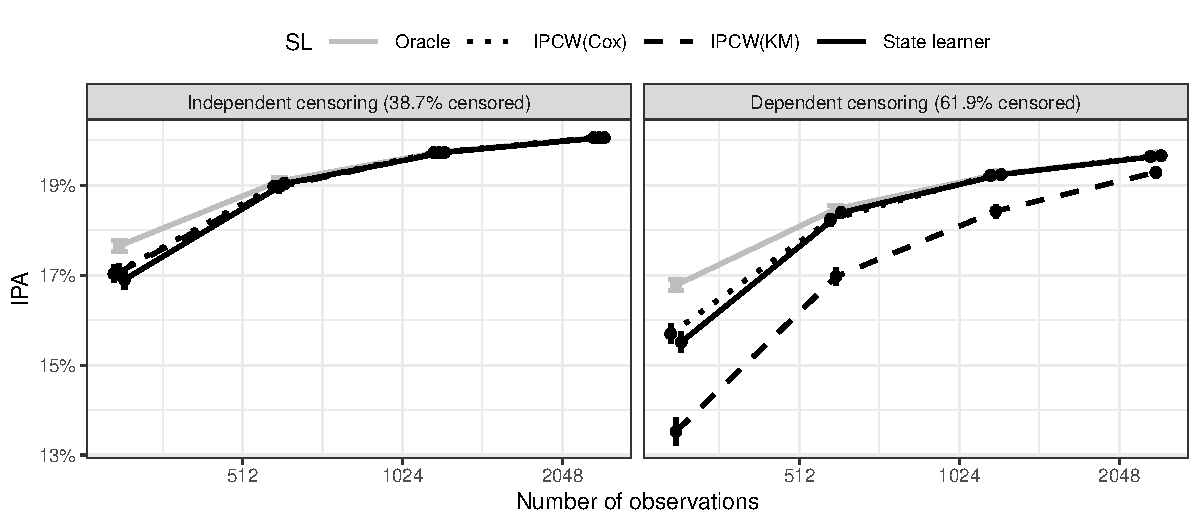
\includegraphics[width=13cm]{experiment-fig-sl-ipcw}
  \caption{For the risk prediction models provided by each of the
    super learners, the IPA is plotted against sample size. The
    results are averages across 1000 simulated data sets and the error
    bars are used to quantify the Monte Carlo uncertainty. JSSL
    denotes the joint survival super learner. }
\label{fig:ipcw-fail}
\end{figure}
 
For the second aim, we consider the super learner {\it survSL}
proposed by \citep{westling2021inference} which like the joint
survival super learner does not require a pre-specified censoring
model. Both methods provide estimates of the event-time and censoring
distributions and hence we compare their performance with respect to
both the outcome and the censoring distribution. Again we use the IPA
to quantify the predictive performance.

The results for the second aim are shown in
Figures~\ref{fig:zelefski-out} and~\ref{fig:zelefski-cens}. We see
that for most sample sizes, the joint survival super learner has
similar or higher IPA compared to survSL with respect to both the
prediction of the censoring and the outcome risks. We note that the
advantage of the joint survival super learner in this particular
simulation setting might be due that it is a discrete super learner,
whereas survSL combines the learners.


\begin{figure}[ht]
  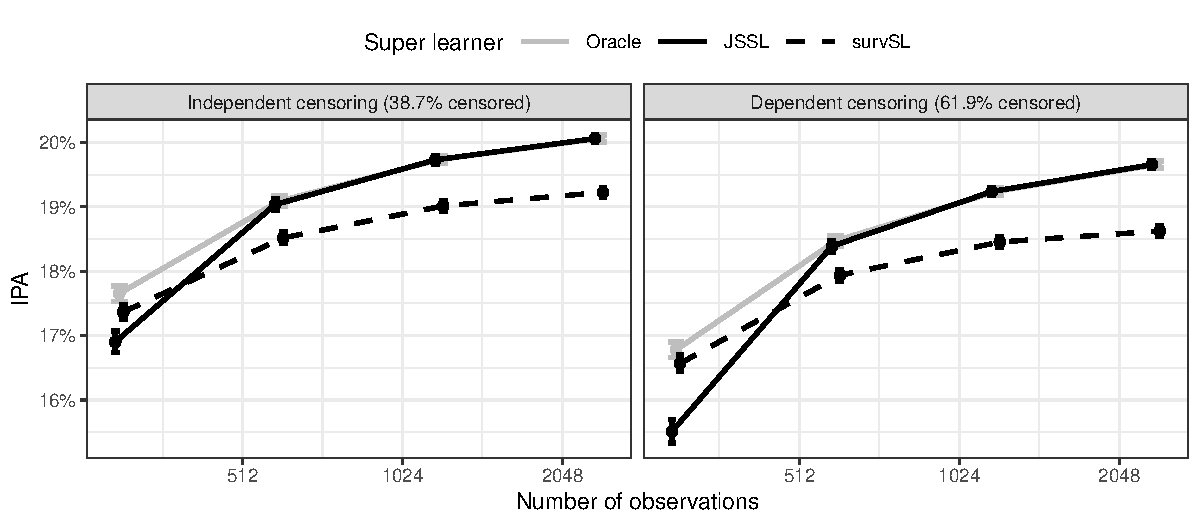
\includegraphics[width=13cm]{experiment-fig-sl-survSL-out}
\caption{For the risk prediction models of the outcome provided by
  each of the super learners, the IPA at the fixed time horizon is
  plotted against sample size. The results are averages across 1000
  repetitions and the error bars are used to quantify the Monte Carlo
  uncertainty. JSSL denotes the joint survival super learner.}
\label{fig:zelefski-out}
\end{figure}


\begin{figure}[ht]
  \begin{center}
      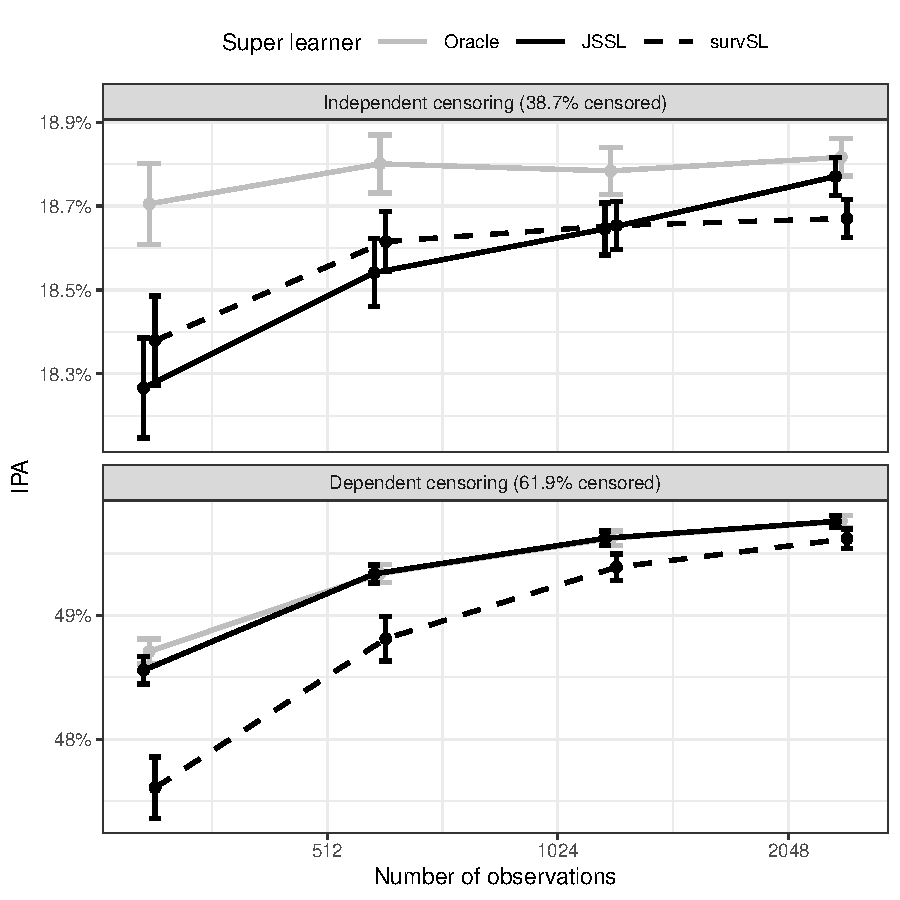
\includegraphics[width=10cm]{experiment-fig-sl-survSL-cens}
  \end{center}
\caption{For the risk prediction models of the censoring model
    provided by each of the super learners, the IPA at the fixed time
    horizon is plotted against sample size. The results are averages
    across 1000 repetitions and the error bars are used to quantify
    the Monte Carlo uncertainty. JSSL denotes the joint survival super
    learner.}
\label{fig:zelefski-cens}
\end{figure}

\section{Prostate cancer study}
\label{sec:real-data-appl}

We use the prostate cancer data of \cite{kattan2000pretreatment} to
illustrate the use of the joint survival super learner in the presence
of competing risks. We have introduced the data in
Section~\ref{sec:numer-exper}. The data consist of 1,042 patients who
are followed from start of followup until tumour recurrence ($n=268$),
death without tumour recurrence ($n=29$), or censored ($n=745$),
whatever came first. We use the joint survival super learner to rank
libraries of learners for the cause-specific cumulative hazard
functions of tumour recurrence, death without tumour recurrence, and
censoring. The three libraries of learners each include five learners:
the Nelson-Aalen estimator, three Cox regression models (unpenalized,
lasso, elastic net) each including additive effects of the baseline
covariates, and a random survival forest. The Nelson-Aalen estimator
is estimated without covariates and serves as a benchmark model which
guarantees that the joint survival super learner is not worse than a
model which predicts the same probability to all individuals. The
other four learners use the five baseline covariates listed in
Section~\ref{sec:numer-exper} to predict the three cumulative hazard
functions of time to tumour recurrence \( \Lambda_1 \), time to death
without tumour recurrence \( \Lambda_2 \), and time to censoring
$\Gamma$. The resulting library consists of \( 5^3 = 125 \)
learners. We use five folds for training and testing the models,
repeat training and evaluation five times with different splits, and
obtain the discrete joint survival super learner as the combination
with the best average five-fold integrated Brier score across the five
repetitions. Table \ref{tab:1} shows integrated Brier scores for the
conditional state occupation probability function \( F \) as defined
in Section~\ref{sec:joint-survival-super-learner}, evaluated 3 years
after randomization for a selection of the 125 learners. We see that
among the five best combinations, the random survival forest is always
selected for \(\Gamma\) and that the differences for different
learners of \(\Lambda_1\) and \(\Lambda_2\) are small. To illustrate
the comparative performance of the discrete joint survival super
learner, we also split the data randomly into a training set with
\(n=658\) individuals and a test set with the remaining \(n=384\)
individuals.  We fit the discrete joint survival super learner (five
repetitions of five-fold cross-validation) and for comparison
pre-specified cause-specific Cox regression models to the training
set. In the training set, the discrete joint survival super learner
chooses the unpenalized Cox regression model for tumor recurrence, the
elastic net Cox regression for death without tumor recurrence, and the
random survival forest for censoring. Figure \ref{fig:zelefski-real}
compares the 3-year risk predictions from the pre-specified Cox model
and the discrete joint survival super learner in the test set.

\begin{table}[ht]
  \caption{The results of applying the 125 combinations of learners to
the prostate cancer data set. Shown are the best 5 combinations and
selected intermediate ranks.  The `Loss' is the integrated Brier
score evaluated at 3 years and `SD' is the standard deviation
across the five repetitions of five-fold cross-validation. The discrete
joint survival super learner chooses rank 1. }
\begin{center}  
\begin{tabular}{ l| c c c c c } 
  Rank&Cause 1&Cause 2&Censored&Loss&SD \\\hline
  $   1 $&elastic net&elastic net&random forest&$  7.0205 $&$ 0.030977 $ \\
  $   2 $&lasso&elastic net&random forest&$  7.0209 $&$ 0.031035 $ \\
  $   3 $&Cox&elastic net&random forest&$  7.0224 $&$ 0.030871 $ \\
  $   4 $&elastic net&lasso&random forest&$  7.0225 $&$ 0.030170 $ \\
  $   5 $&lasso&lasso&random forest&$  7.0228 $&$ 0.030237 $ \\
  $  25 $&random forest&random forest&lasso&$  7.3845 $&$ 0.026975 $ \\
  $  50 $&elastic net&random forest&lasso&$  7.3974 $&$ 0.021290 $ \\
  $  75 $&lasso&Cox&lasso&$  7.4059 $&$ 0.024660 $ \\
  $ 100 $&Nelson-Aalen&Cox&elastic net&$  7.8300 $&$ 0.016719 $ \\
  $ 125 $&Nelson-Aalen&Nelson-Aalen&Nelson-Aalen&$ 10.3298 $&$ 0.003289 $ \\
\end{tabular}\label{tab:1}
\end{center}
\end{table}


\begin{figure}[ht]
  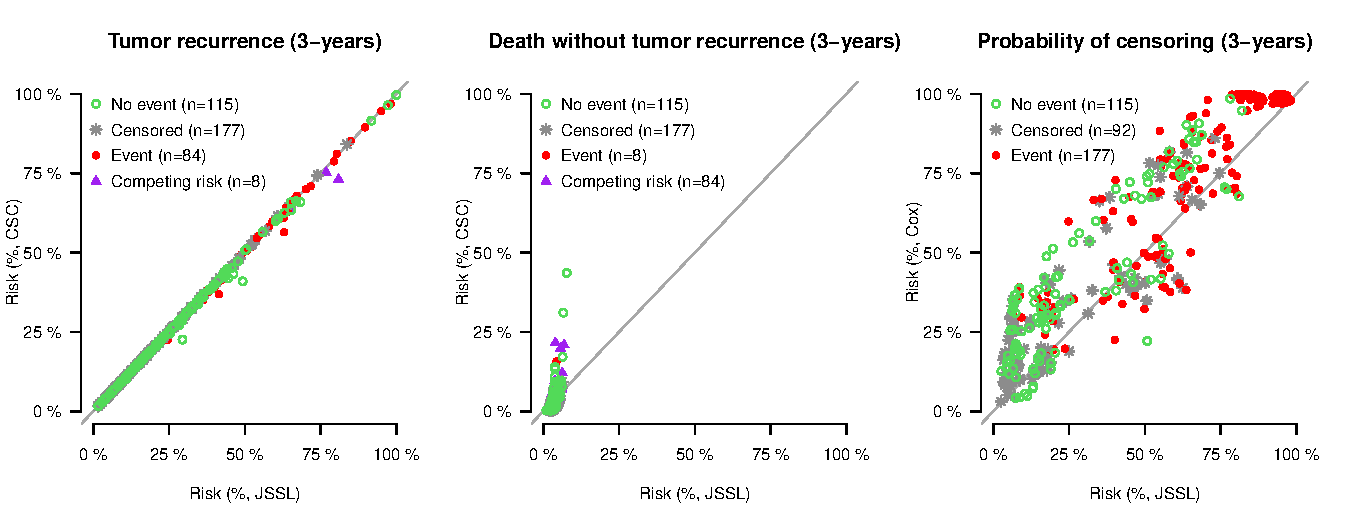
\includegraphics[width=14cm]{risks_zelefsky_single.pdf}
 \caption{Comparison of risk predictions of the discrete joint
   survival super learner and pre-specified Cox regressions in an
   independent test data set.}
\label{fig:zelefski-real}
\end{figure}


\section{Discussion}
\label{sec:discussion}

A major advantage of the joint survival super learner is that the
performance of each combination of learners can be estimated without
additional nuisance parameters. A potential drawback of our approach
is that we are evaluating the loss of the learners on the level of the
observed data distribution, while the target of the analysis is either
the event-time distribution, or the censoring distribution, or
both. Our numerical experiments suggest that our approach does provide
estimates of the conditional survival functions which perform well,
also when the predictive performance is measured against the true
survival function with no censoring present.

Alternatives to using a performance measure defined with respect the
observed data are the use of IPCW loss functions, censoring unbiased
transformations, or pseudo-values. As mentioned in
Section~\ref{sec:super-learning}, the drawback of these approaches is
that they all need a pre-specified estimator of the censoring
distribution, and hence these methods are not immediately applicable
if we do not in advance know how to model the censoring
distribution. We note that for the special case where the partial
log-likelihood loss can be used, this loss function, like our
suggested approach, also measures performance with respect to a
feature defined by the observed data distribution
\citep[e.g.,][]{hjort1992inference,whitney2019comment}. We do not know
of any method that would allow us to evaluate performance of a
risk-prediction model in censored data without either modeling
additional nuisance parameters (such as the censoring distribution) or
measuring performance directly with respect to the observed data.

A relevant application of the joint survival super learner is within
the framework of targeted learning \citep{van2011targeted}, also known
as debiased machine learning \citep{chernozhukov2018double}, -- a
general methodology that combines flexible, data-adaptive estimation
of nuisance parameters with asymptotically valid inference for
low-dimensional target parameters.  For example, the methods in
\cite{van2003unified} and \cite{rytgaard2022targeted} target the
average treatment effect in a survival setting, which require
estimates of the cause-specific cumulative hazard functions and the
censoring cumulative hazard function. The joint survival super learner
can be used to estimate these nuisance parameters and is more
generally well suited for targeted and debiased machine learning with
right-censored data.

We have focused on a discrete version of the joint survival super
learner, but it is of interest to extend the method to a proper
ensemble learner, where learners are combined, e.g., through
stacking. There are at least two possible directions for constructing
an ensemble version of the joints survival super leaner. One option is
to construct a single convex combination of the F-learners
\( \phi \in \Phi(\mathcal{A}_1, \mathcal{A}_2, \mathcal{B})
\). Another, perhaps more interesting option, is to construct three
separate convex combinations of the learners in \( \mathcal{A}_1 \),
\( \mathcal{A}_2 \), and \( \mathcal{B} \).  How such an ensemble
should be build and implemented is an interesting topic for future
research.

[Generalizing our proposal to ensemble learning is ... At least two
   strategies could be pursued. First, ensemble for F. More
   interestingly, jointly build ensembles for all element of the tuple.]


\appendix

\section*{Appendix}


Define
\( \bar{B}_{\tau,P}(F, o) = \bar{B}_{\tau}(F, o) -
\bar{B}_{\tau}(F_P, o) \) and
\( R_{P}(F) = \E_P{[\bar{B}_{\tau,P}(F, O)]} \), where the
integrated Brier score \( \bar{B}_{\tau} \) was defined in
Section~\ref{sec:joint-survival-super-learner}. Recall the norm
\( \Vert \blank \Vert_{P}\) defined in
equation~(\ref{eq:norm}).

\begin{lemma}
  \label{lemma:norm}
  \( R_{P}(F) = \Vert F - F_P \Vert_{P}^2 \).
\end{lemma}
\begin{proof}
  For any \( t \in [0, \tau] \) and \( l\in \{-1,0,1,2\} \) we have
  \begin{align*}
    & \E_{P}{\left[ (F(t, l, X) - \1{\{\eta(t) = l \}})^2 \right]}
    \\
    & =    \E_{P}{\left[ (F(t, l, X) - F_P(t, l, X) + F_P(t, l, X) - \1{\{\eta(t) = l
      \}})^2 \right]}
    \\
    & =    \E_{P}{\left[ (F(t, l, X) - F_P(t, l, X))^2\right]}
      + \E_{P}{\left[ (F_P(t, l, X) - \1{\{\eta(t) = l \}})^2\right]}
    \\
    & \quad
      + 2\E_{P}{\left[ (F(t, l, X) - F_P(t, l, X))(F_P(t, l, X) - \1{\{\eta(t) = l
      \}})\right]}
    \\
    & =    \E_{P}{\left[ (F(t, l, X) - F_P(t, l, X))^2\right]}
      + \E_{P}{\left[ (F_P(t, l, X) - \1{\{\eta(t) = l \}})^2\right]},
  \end{align*}
  where the last equality follows from the tower property. Hence, using Fubini,
  we have
  \begin{equation*}
    \E_P{[\bar{B}_{\tau}(F, O)]}
    = \Vert F - F_P \Vert_{P}^2 + \E_P{[\bar{B}_{\tau}(F_P, O)]}.
  \end{equation*}
\end{proof}

\begin{proof}[of Proposition~\ref{prop:stric-prop}]
  The result follows from Lemma~\ref{lemma:norm}.
\end{proof}

Recall that we use \( \Phi_n \) to denote a library of learners for the
function \( F \), and that \( \hat{\phi} \) and \( \tilde{\phi} \) denotes,
respectively, the discrete super learner and the oracle learner for the library
\( \Phi_n \), c.f., Section~\ref{sec:joint-survival-super-learner}.

\begin{proof}[of Proposition~\ref{prop:oracle-prop}]
  Minimizing the loss \( \bar{B}_{\tau} \) is equivalent to
  minimizing the loss \( \bar{B}_{\tau,P} \), so the discrete super learner and
  oracle according to \( \bar{B}_{\tau} \) and \( \bar{B}_{\tau,P} \) are
  identical. By Lemma~\ref{lemma:norm}, \( R_P(F) \geq 0 \) for any
  \( F \in \mathcal{F}_{\mathcal{P}} \), and so using Theorem 2.3 from
  \citep{vaart2006oracle} with \( p=1 \), we have that for all \( \delta >0 \),
\begin{align*}
  & \frac{1}{K} \sum_{k=1}^{K} \E_{P}{\left[ R_P(\hat{\phi}_n(\data_n^{-k})) \right]}
  \\
  &  \quad \leq
    (1+2\delta)\frac{1}{K} \sum_{k=1}^{K}\E_{P}{\left[ R_P(\tilde{\phi}_n(\data_n^{-k})) \right]}
  \\
  & \qquad + (1+\delta) \frac{16 K}{n}
    \log(1 + |\Phi_n|)\sup_{F \in \mathcal{F}_{\mathcal{P}}}
    \left\{
    M(F) + \frac{v(F)}{R_P(F)}
    \left(
    \frac{1}{\delta} + 1
    \right)
    \right\}
\end{align*}
where for each \( F \in \mathcal{F}_{\mathcal{P}} \),
\( (M(F), v(F)) \) is some Bernstein pair for the function
\(o \mapsto \bar{B}_{\tau,P}(F, o) \). As
\( \bar{B}_{\tau,P}(F, \blank) \) is uniformly bounded by \( \tau \)
for any \( F \in \mathcal{F}_{\mathcal{P}} \), it follows from section
8.1 in \citep{vaart2006oracle} that
\( (\tau, 1.5 \E_P{[\bar{B}_{\tau,P}(F, O)^2]}) \) is a Bernstein
pair for \( \bar{B}_{\tau,P}(F, \blank) \). Now, for any
\( a,b,c \in \R \) we have
\begin{align*}
  (a-c)^2 - (b-c)^2
  & = (a-b+b-c)^2 - (b-c)^2
  \\
  & = (a-b)^2 + (b-c)^2 +2(b-c)(a-b) - (b-c)^2
  \\
  & = (a-b)
    \left\{
    (a-b) +  2(b-c)
    \right\}
  \\
  & = (a-b)
    \left\{
     a + b -2c
    \right\},
\end{align*}
so using this with \( a=F(t, l, x) \), \( b=F_P(t, l, x) \), and
\( c = \1{\{\eta(t) = l\}} \), we have by Jensen's inequality
\begin{align*}
  & \E_P{[\bar{B}_{\tau,P}(F, O)^2]}
  \\
  & \leq
    2\tau\E_{P}{\left[
    \sum_{l=-1}^{2} \int_0^{\tau}
    \left\{
    \left(
    F(t, l, X) - \1{\{\eta(t) = l\}}
    \right)^2
    -
    \left(
    F_P(t, l, X) - \1{\{\eta(t) = l\}}
    \right)^2
    \right\}^2
    \diff t 
    \right]}
  \\
  & =2\tau
    \E_{P}\Bigg[
    \sum_{l=-1}^{2} \int_0^{\tau}
    \left(
    F(t, l, X) - F_P(t, l, X)
    \right)^2
  \\
  & \quad \quad \quad\quad \quad \quad \times
    \left\{
    F(t, l, X) +  F_P(t, l, X)-2 \1{\{\eta(t) = l\}}
    \right\}^2
    \diff t 
    \Bigg]
  \\
  & \leq
    8\tau \E_{P}{\left[
    \sum_{l=-1}^{2} \int_0^{\tau}
    \left(
    F(t, l, X) - F_P(t, l, X)
    \right)^2
    \diff t 
    \right]}.
  \\
  & =
    8\tau \Vert F - F_P \Vert_{P}^2.
\end{align*}
Thus when \( v(F) = 1.5 \E_P{[\bar{B}_{\tau,P}(F, O)^2]} \) we have by
Lemma~\ref{lemma:norm}
\begin{equation*}
  \frac{v(F)}{R_P(F)}
  = 1.5 \frac{\E_P{[\bar{B}_{\tau,P}(F, O)^2]}}{\E_P{[\bar{B}_{\tau,P}(F, O)]}}
  \leq 12 \tau,
\end{equation*}
and so using the Bernstein pairs \( (\tau, 1.5 \E_P{[\bar{B}_{\tau,P}(F, O)^2]}) \) we have
\begin{equation*}
  \sup_{F \in \mathcal{F}_{\mathcal{P}}}
  \left\{
    M(F) + \frac{v(F)}{R_P(F)}
    \left(
      \frac{1}{\delta} + 1
    \right)
  \right\}
  \leq \tau
  \left(
    13 + \frac{12}{\delta}
  \right).
\end{equation*}
For all $\delta>0$ we thus have
\begin{align*}
  \frac{1}{K} \sum_{k=1}^{K} \E_{P}{\left[ R_P(\hat{\phi}_n(\data_n^{-k})) \right]}
  \leq
  &(1+2\delta)\frac{1}{K} \sum_{k=1}^{K}\E_{P}{\left[ R_P(\tilde{\phi}_n(\data_n^{-k})) \right]}
  \\
  & \quad
    + (1+\delta)\log(1 + |\Phi_n|) \tau \frac{16 K}{n}
    \left(
    13 + \frac{12}{\delta}
    \right),
\end{align*}
which is equivalent to
\begin{align*}
   \E_{P}{\left[ R_P(\hat{\phi}_n(\data_n^{-k})) \right]}
  \leq
  &(1+2\delta) \E_{P}{\left[ R_P(\tilde{\phi}_n(\data_n^{-k})) \right]}
  % \\
  % &
    \quad
    + (1+\delta)\log(1 + |\Phi_n|) \tau \frac{16 K}{n}
    \left(
    13 + \frac{12}{\delta}
    \right),
\end{align*}
for any \( k\in \{1, \dots, K\} \), because we have assumed that
\( |\data_n^{-k}| = n/K \) for all \( k \), and hence the expectations
on the right- and left-hand side above do not depend on \( k \). The
final result then follows from Lemma~\ref{lemma:norm}.
\end{proof}

\begin{proof}[of Corollary~\ref{cor:asymp-cons}]
  By definition of the oracle and Lemma~\ref{lemma:norm},
  \begin{equation*}
    \frac{1}{K} \sum_{k=1}^{K} \E_{P}{\left[ \Vert \tilde{\phi}_n(\data_n^{-k}) - F_P \Vert_{P}^2
      \right]} \leq
    \frac{1}{K} \sum_{k=1}^{K}\E_{P}{\left[ \Vert
        \phi_n(\data_n^{-k}) - F_P \Vert_{P}^2
      \right]}
    =
    \E_{P}{\left[ \Vert \phi_n(\data_n^{-k}) - F_P \Vert_{P}^2
      \right]},
  \end{equation*}
  for all \( n \in \N \), where the last equality follows because all
  the training sets \( \data_n^{-k} \) have the same distribution. The
  result then follows from Proposition~\ref{prop:oracle-prop} by
  letting $\delta$ grow to zero with \( n \), for instance as
  $\delta_n = \log(n)^{-\epsilon}$ for some $\epsilon>0$.
\end{proof}




\bibliography{bib.bib}


\end{document}
